\newcommand{\VBGBar}{\overline{\vb G}}
\newcommand{\KB}{\vb k\subt{B}}

%%%%%%%%%%%%%%%%%%%%%%%%%%%%%%%%%%%%%%%%%%%%%%%%%%%%%%%%%%%%%%%%%%%%%%
%%%%%%%%%%%%%%%%%%%%%%%%%%%%%%%%%%%%%%%%%%%%%%%%%%%%%%%%%%%%%%%%%%%%%%
%%%%%%%%%%%%%%%%%%%%%%%%%%%%%%%%%%%%%%%%%%%%%%%%%%%%%%%%%%%%%%%%%%%%%%
\newpage
\section{Periodic Boundary Conditions}

%%%%%%%%%%%%%%%%%%%%%%%%%%%%%%%%%%%%%%%%%%%%%%%%%%%%%%%%%%%%%%%%%%%%%
%%%%%%%%%%%%%%%%%%%%%%%%%%%%%%%%%%%%%%%%%%%%%%%%%%%%%%%%%%%%%%%%%%%%%
%%%%%%%%%%%%%%%%%%%%%%%%%%%%%%%%%%%%%%%%%%%%%%%%%%%%%%%%%%%%%%%%%%%%%
\subsection{PBC BEM formulations}

%=================================================
%=================================================
%=================================================
\subsubsection{Scattered field of an infinite PEC surface}

Consider the scattered field produced by an 
induced surface-current density $\vb K(\vb x)$ on
an infinite PEC surface $\mc S_\infty$:
%====================================================================%
\begin{align}
  \vb E\sups{scat}(\vb x)
&=
  \int_{\mc S_\infty} 
   \BG\supt{EE}(\vb x, \vb x^\prime)
   \cdot 
   \vb K(\vb x^\prime)d\vb x^\prime
\\
&=
  ikZ_0
  \int_{\mc S_\infty} 
   \vb G(\vb x, \vb x^\prime) 
   \cdot 
   \vb K(\vb x^\prime)d\vb x^\prime
\label{EScatPBC}
\end{align}
where $k=\omega/c$ ($\omega$ is the angular frequency
at which we are working) and $Z_0$ is the impedance
of free space (assume we are in vacuum for now).
If we now suppose that 
%====================================================================%
\begin{itemize}
 \item the surface $\mc S_\infty$ consists of an infinite lattice
       of copies of a unit-cell surface $\mc S_0$ translated through
       two-dimensional lattice vectors of the form 
       \numeq{LatticeVectors}{\vb L=n_1 \vb L_1 + n_2\vb L_2}
       and
 \item the surface current respects this periodicity in the 
       Bloch sense, i.e. we have
       $$ \vb K\sups{inc}(\vb x+\vb L)
          = e^{i\KB \cdot \vb L} \, \vb K\sups{inc}(\vb x)
       $$
       for some Bloch vector $\KB$
\end{itemize}
%====================================================================%
then I can write the scattered field (\ref{EScatPBC}) as an integral
over just the unit cell:
%====================================================================%
\begin{align}
   \vb E\sups{scat}(\vb x)
&= ikZ_0 
   \sum_{\vb L}
   \int_{\mc S_0}
   \vb G(\vb x, \vb x^\prime+\vb L)
   \cdot 
   \vb K(\vb x^\prime + \vb L ) \, d\vb x^\prime
\nn
&= ikZ_0
   \int_{\mc S_0}
   \underbrace{
   \left\{
   \sum_{\vb L}
   e^{i\KB \cdot \vb L}
   \vb G(\vb x, \vb x^\prime+\vb L)
   \right\}
              }_{\VBGBar(\vb x, \vb x^\prime)}
   \cdot 
   \vb K(\vb x^\prime) \, d\vb x^\prime
\nn
&= ikZ_0 
   \int_{\mc S_0}
   \VBGBar(\vb x, \vb x^\prime)
   \cdot 
   \vb K(\vb x^\prime) \, d\vb x^\prime
\label{EScatPBC}
\end{align}
where $\VBGBar$ is the dyadic periodic Green's function,
whose properties we now discuss.

%%%%%%%%%%%%%%%%%%%%%%%%%%%%%%%%%%%%%%%%%%%%%%%%%%%%%%%%%%%%%%%%%%%%%%
%%%%%%%%%%%%%%%%%%%%%%%%%%%%%%%%%%%%%%%%%%%%%%%%%%%%%%%%%%%%%%%%%%%%%%
%%%%%%%%%%%%%%%%%%%%%%%%%%%%%%%%%%%%%%%%%%%%%%%%%%%%%%%%%%%%%%%%%%%%%%
\subsubsection{Periodic Green's functions}
The dyadic periodic Green's function introduced in 
(\ref{EScatPBC}) is 
%====================================================================%
\begin{align*}
 \VBGBar(\vb x, \vb x^\prime)
&=\sum_{\vb L} e^{i\KB \cdot \vb L}\vb G(\vb x, \vb x^\prime+\vb L)
\intertext{with cartesian components}
 \GBar_{ij}(\vb x, \vb x^\prime)
&=\sum_{\vb L} e^{i\KB \cdot \vb L}G_{ij}(\vb x, \vb x^\prime+\vb L)
\\
&=\sum_{\vb L} 
   e^{i\KB \cdot \vb L} 
  \left[
   \Big( \delta_{ij} + \frac{1}{k^2}\partial_i \partial_j\Big)
   \frac{e^{ik|\vb x - \vb x^\prime - \vb L|}}
        {4\pi|\vb x - \vb x^\prime - \vb L|}
  \right]
\intertext{Interchange differentiation and summation:}
&=
  \Big( \delta_{ij} + \frac{1}{k^2}\partial_i \partial_j\Big)
  \underbrace{
  \left\{ \sum_{\vb L} 
          e^{i\KB \cdot \vb L}
          \frac{e^{ik|\vb x - \vb x^\prime - \vb L|}} 
          {4\pi|\vb x - \vb x^\prime - \vb L |}
   \right\}}_{\GBar_0(\vb x-\vb x^\prime)}
\end{align*}
where $\GBar_0$ is the scalar periodic Green's function.
(\lss computes $\GBar_0$ and its derivatives using Ewald
summation together with an interpolation-table method
discussed below.)
%====================================================================%

\paragraph{Symmetries of $\VBGBar$}

Suppose the lattice basis vectors are $\vb L_1, \vb L_2$.
Then we can write the sum that defines the scalar periodic Green's
function in the form
%====================================================================%
\begin{align*}
\GBar_0(\vb r)
&= \sum_{n_1, n_2=-\infty}^\infty 
   e^{i\KB \cdot(n_1 \vb L_1 + n_2 \vb L_2)}
     G_0(\vb r - n_1\vb L_1 - n_2 \vb L_2)
\end{align*}
%====================================================================%
Now consider evaluating $\GBar$ at an argument displaced
through one full lattice basis vector:
\begin{align*}
 \VBGBar(\vb r + \vb L_1) 
&= \sum_{n_1, n_2=-\infty}^\infty 
   e^{i\KB \cdot (n_1\vb L_1 + n_2\vb L_2)}
   G_0( \vb r + \vb L_1 - n_1 \vb L_1 - n_2 \vb L_2)
\intertext{Add and subtract $\vb L_1$ in the exponent of 
           the Bloch factor:}
&= e^{i\KB \cdot \vb L_1}
   \sum_{n_1, n_2=-\infty}^\infty 
   e^{i\KB \cdot [(n_1-1)\vb L_1 + n_2\vb L_2]}
   G_0( \vb r -(n_1-1)\vb L_1 - n_2 \vb L_2)
\intertext{Now just redefine $n_1\to n_1-1$ in the infinite sum:}
&= e^{i\KB \cdot \vb L_1} \VBGBar( \vb r ).
\end{align*}
%====================================================================%
More generally, for any lattice vector $\vb L$ I have
$$
 \VBGBar(\vb r + \vb L)
 = e^{i\KB \cdot \vb L}\VBGBar(\vb r).
$$

%=================================================
%=================================================
%=================================================
\subsubsection{Discretized EFIE formulation}

Now consider solving for $\vb K(\vb x)$ in the presence
of illumination by an external Bloch-periodic 
field $\vb E\sups{inc}$.
We suppose that the current distribution in the unit cell 
is represented approximately by an expansion in basis
functions $\{\vb b_\alpha(\vb x)\}:$
%====================================================================%
\numeq{KExpansionPBC}
{\vb K(\vb x) \approx k_\alpha \vb b_\alpha(\vb x).}
%====================================================================%
The electric-field integral equation reads
%====================================================================%
\numeq{EFIE}
{\vb E\sups{scat}_\parallel(\vb x)
   =-\vb E\sups{inc}_\parallel(\vb x).
}
%====================================================================%
As in the usual compact-surface case, inserting (\ref{EScatPBC}) 
and (\ref{KExpansionPBC}) and testing with each element in the set 
$\{\vb b_\alpha\}$ yields a discretized PBC EFIE:
%====================================================================%
\begin{align}
 \sum_{\beta}
 \underbrace{
   \Big \langle \vb b_\alpha \Big|
   ikZ_0\VBGBar    
   \Big| \vb b_\beta \Big\rangle
            }_{\vb M_{\alpha\beta}} 
   k_\beta
&=-\Big \langle \vb b_\alpha \Big | \vb E\sups{inc} \Big\rangle
\label{PBCEFIE}
\end{align}
%====================================================================%
In other words, we obtain a formulation that looks exactly
like the formulation for compact objects, with the only
difference being 

Note that the testing procedure that leads to 
(\ref{PBCEFIE}) is only testing the satisfaction
of equation (\ref{EFIE}) for points $\vb x$
\textit{in the unit cell.} However, the Bloch-periodicity
of the incident and scattered fields ensures that
satisfaction of the equation throughout the unit cell
implies its satisfaction everywhere.

%=================================================
%=================================================
%=================================================
\subsection{PBC geometries in {\sc scuff-em}}

\lss supports Bloch-periodic boundary conditions for
periodically repeated geometries. In this case,

\begin{itemize}
 \item The \texttt{.scuffgeo} file will contain
       a \texttt{LATTICE...ENDLATTICE} section defining 
       between one and three lattice basis vectors 
       $\vb L_1, \vb L_2, \vb L_3.$ (In the present 
       discussion we will consider the common case
       of two-dimensional periodicity, so we have two
       lattice basis vectors $\vb L_1, \vb L_2$.) 
       We assume that $\vb L_1, \vb L_2$ have no 
       component in the $z$ direction.
 \item The only portion of the geometry that is
       meshed is that contained with the ``unit cell.''
 \item We will refer to the lattice cell obtained by 
       displacing the unit cell through displacement 
       vector $\vb L=n_1 \vb L_1 + n_y \vb L_2$ as 
       ``lattice cell $(n_1, n_2)$'' or sometimes
       ``lattice cell $\vb L$''.
 \item All currents and fields in lattice cell $(n_1,n_2)$
       are understood to be equal to the corresponding
       currents and fields in lattice cell $(0,0)$ times
       a Bloch phase factor $e^{i\KB \cdot \vb L}$ where
       $\KB$ is the Bloch wavevector.
\end{itemize}

\subsubsection{Straddlers}

Suppose we are trying to mesh the unit cell
of a square-lattice geometry.
Consider the square mesh shown in the 
upper portion of Figure \ref{NoStraddlerFigure}.
If \lss were given this mesh as a description of a
\textit{compact} surface, it would assign a 
total of 40 basis functions, as indicated by 
the arrows in the lower portion of 
Figure \ref{NoStraddlerFigure}.
In particular, no basis functions would be assigned
to exterior edges. Such a set of basis functions
would have the property that, when we consider
the infinite surface obtained by periodically
replicating the mesh and the basis functions,
no currents could flow from one unit cell to the next;
all currents would be localized within the area of
individual unit cells. 
%####################################################################%
\begin{figure}
\begin{center}
\begin{tabular}{c}
\resizebox{!}{0.5\textheight}{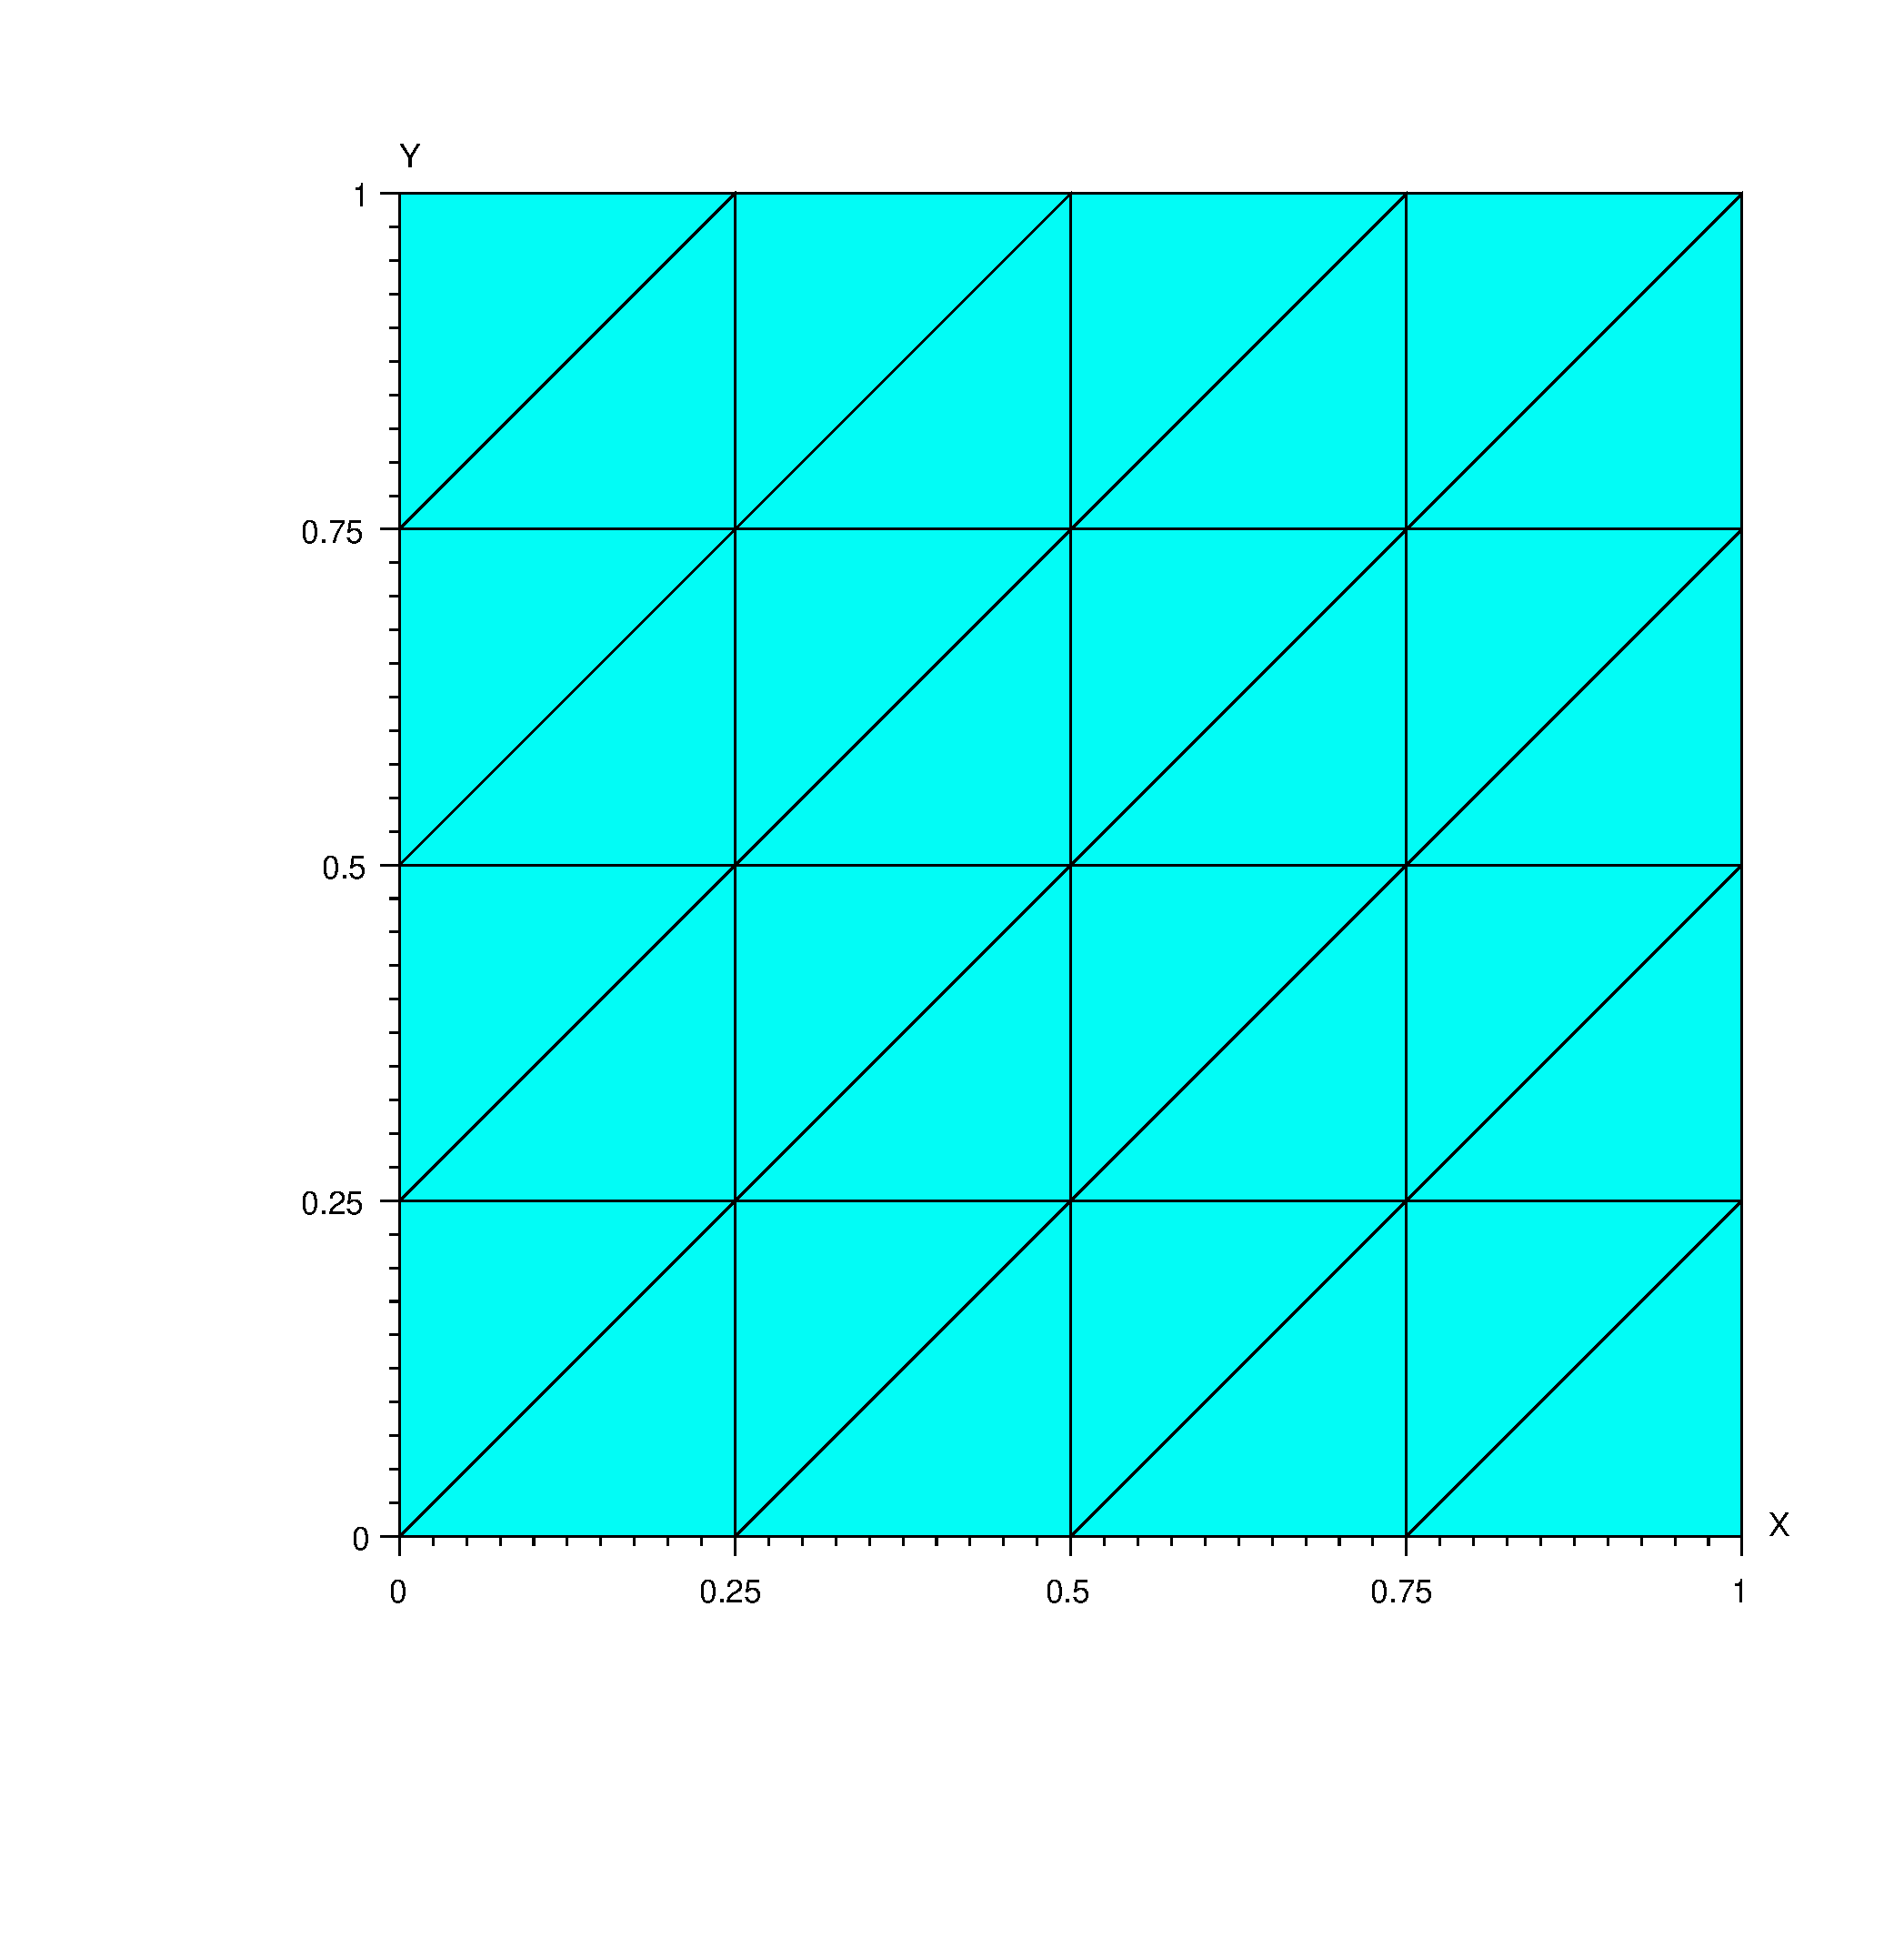
\includegraphics{SquareMesh0.pdf}}
\\[-0.5in]
\hspace{0.45in} \resizebox{!}{0.05\textheight}{$\Downarrow$}
\\[-0.2in]
\resizebox{!}{0.5\textheight}{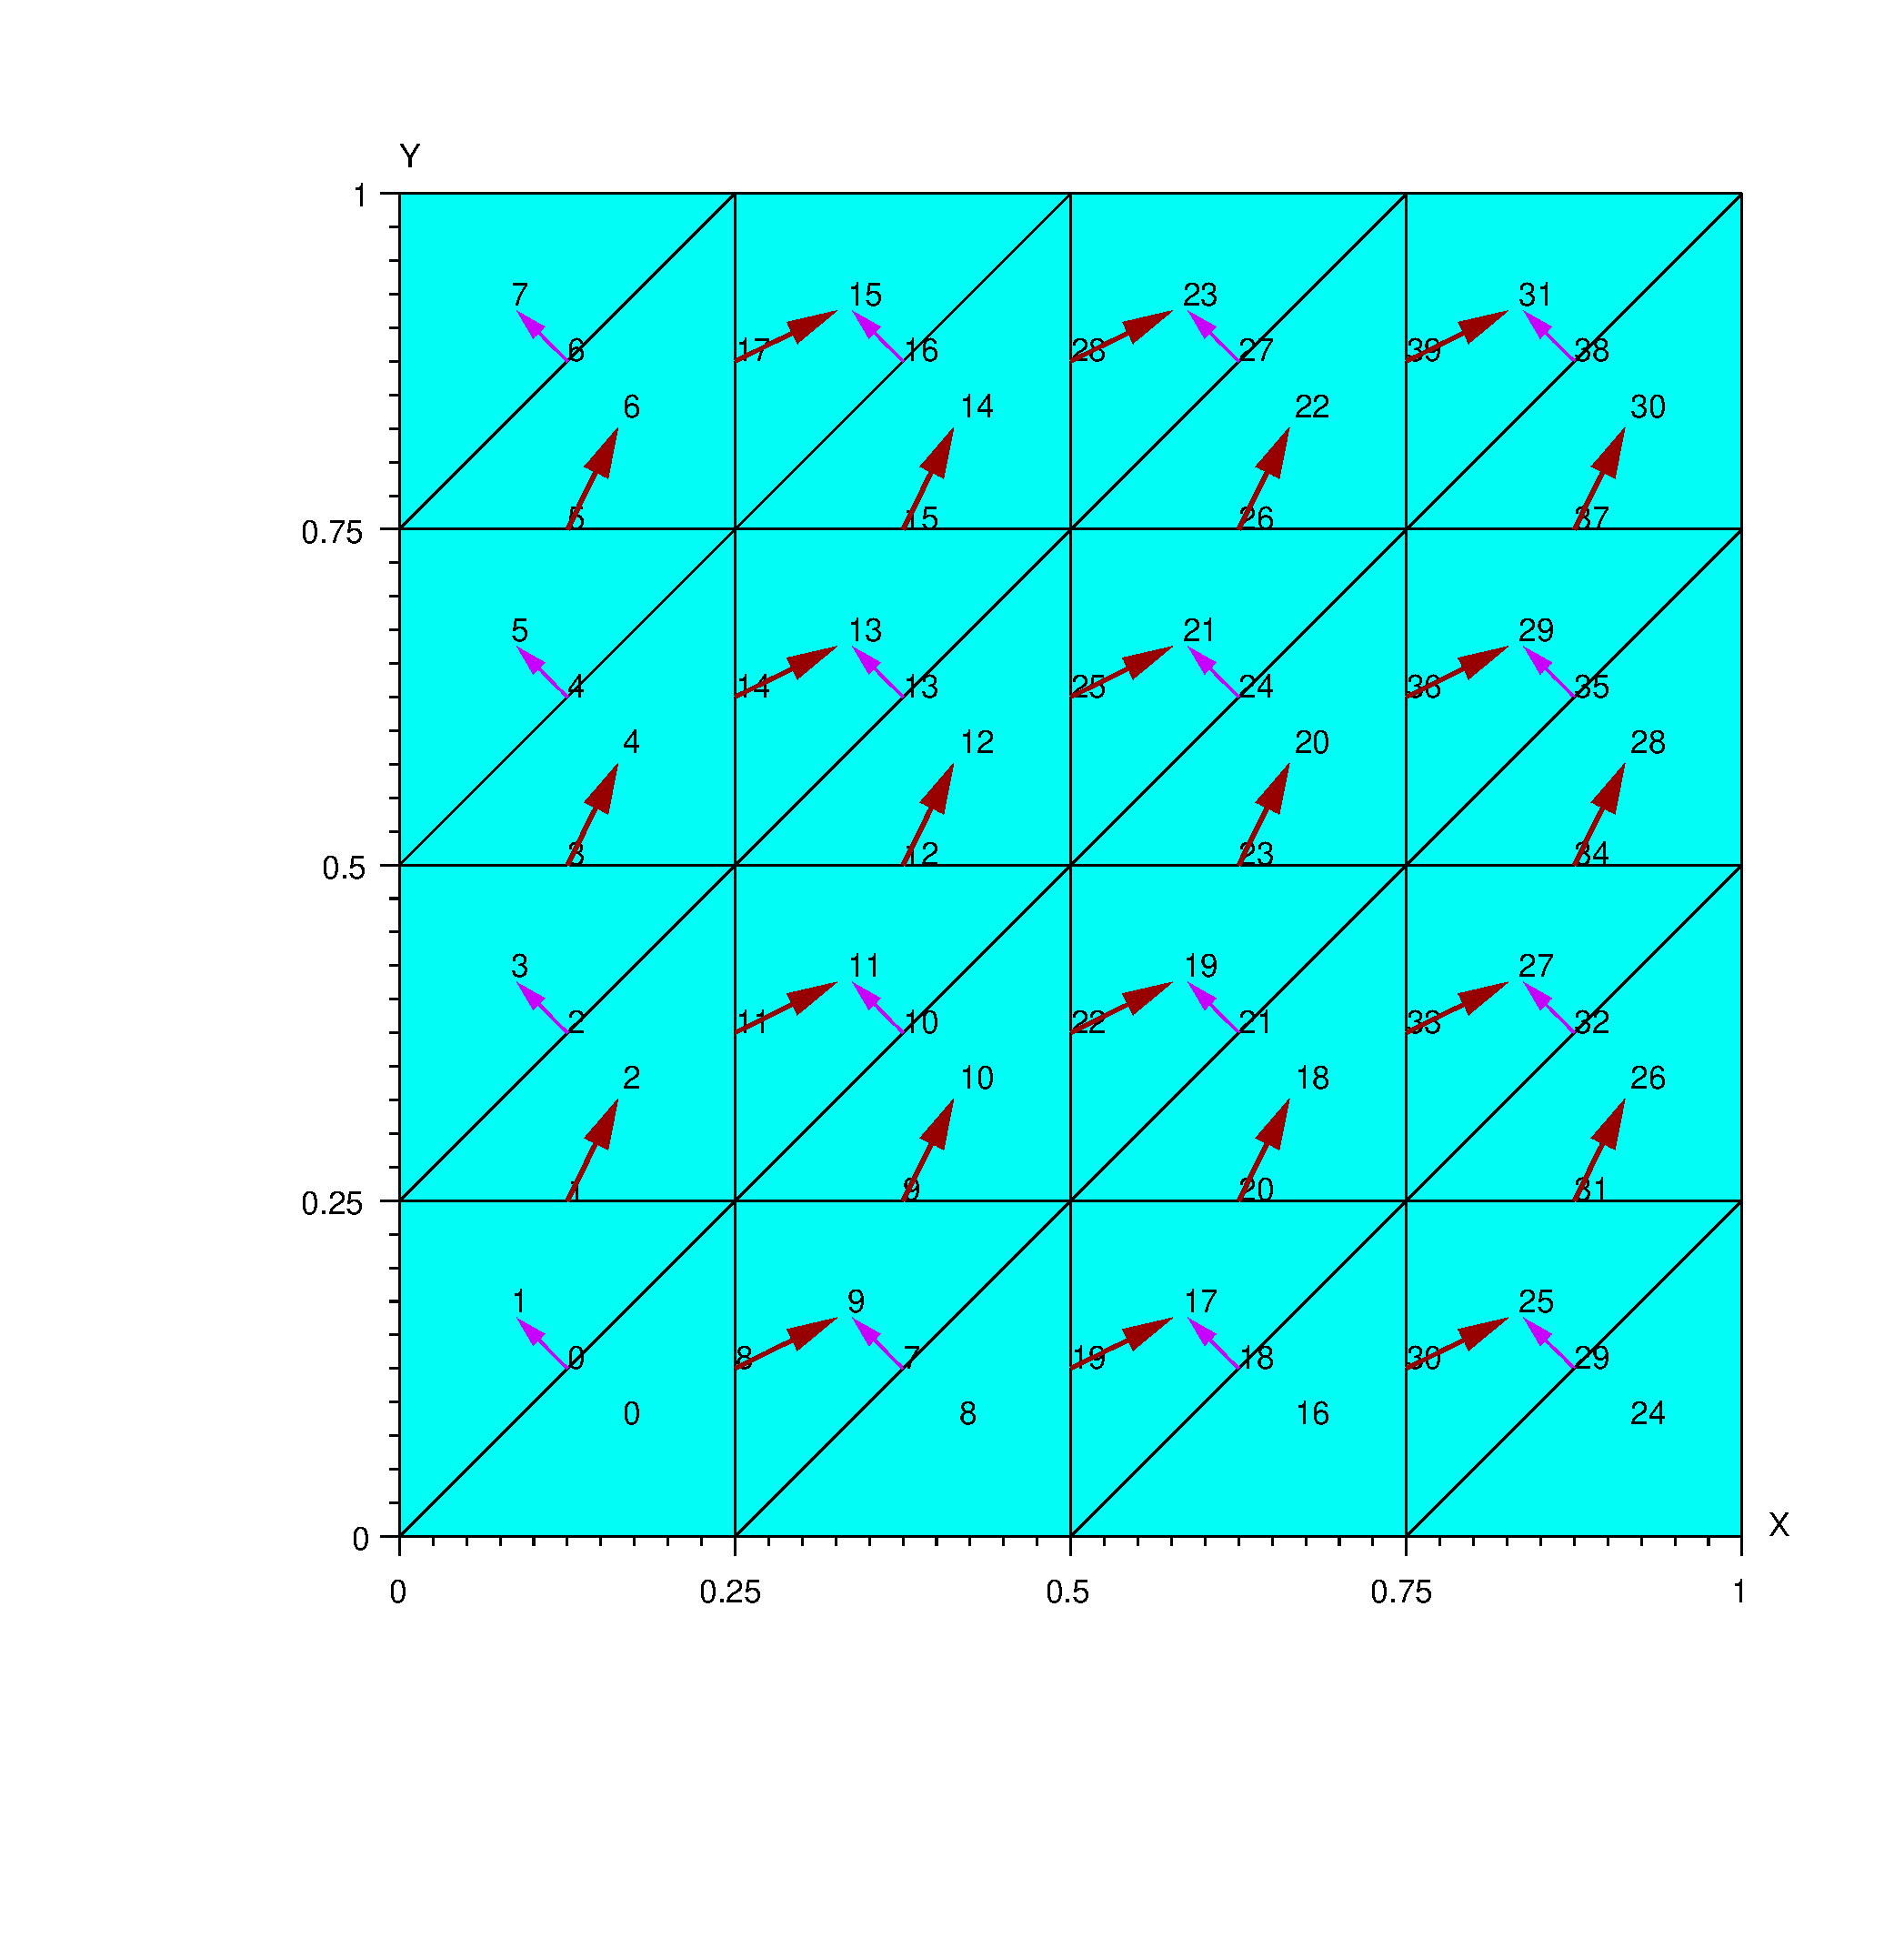
\includegraphics{SquareMesh1.pdf}}
\end{tabular}
\caption{The usual assignment of RWG basis functions 
         to an input surface mesh.
         Integers inside panels denote panel indices.
         Indices lying atop edges denote RWG basis-function indices.
         Arrows indicate directions of current flow.
        } 
\label{NoStraddlerFigure}
\end{center}
\end{figure}
%####################################################################%
To remedy this difficulty, \lss automatically
adds \textit{straddlers} to the surface meshes
specified to the code in geometries involving
extended surfaces. 
This is illustrated in Figure \ref{StraddlerFigure}.
%####################################################################%
\begin{figure}
\begin{center}
\resizebox{\textwidth}{!}{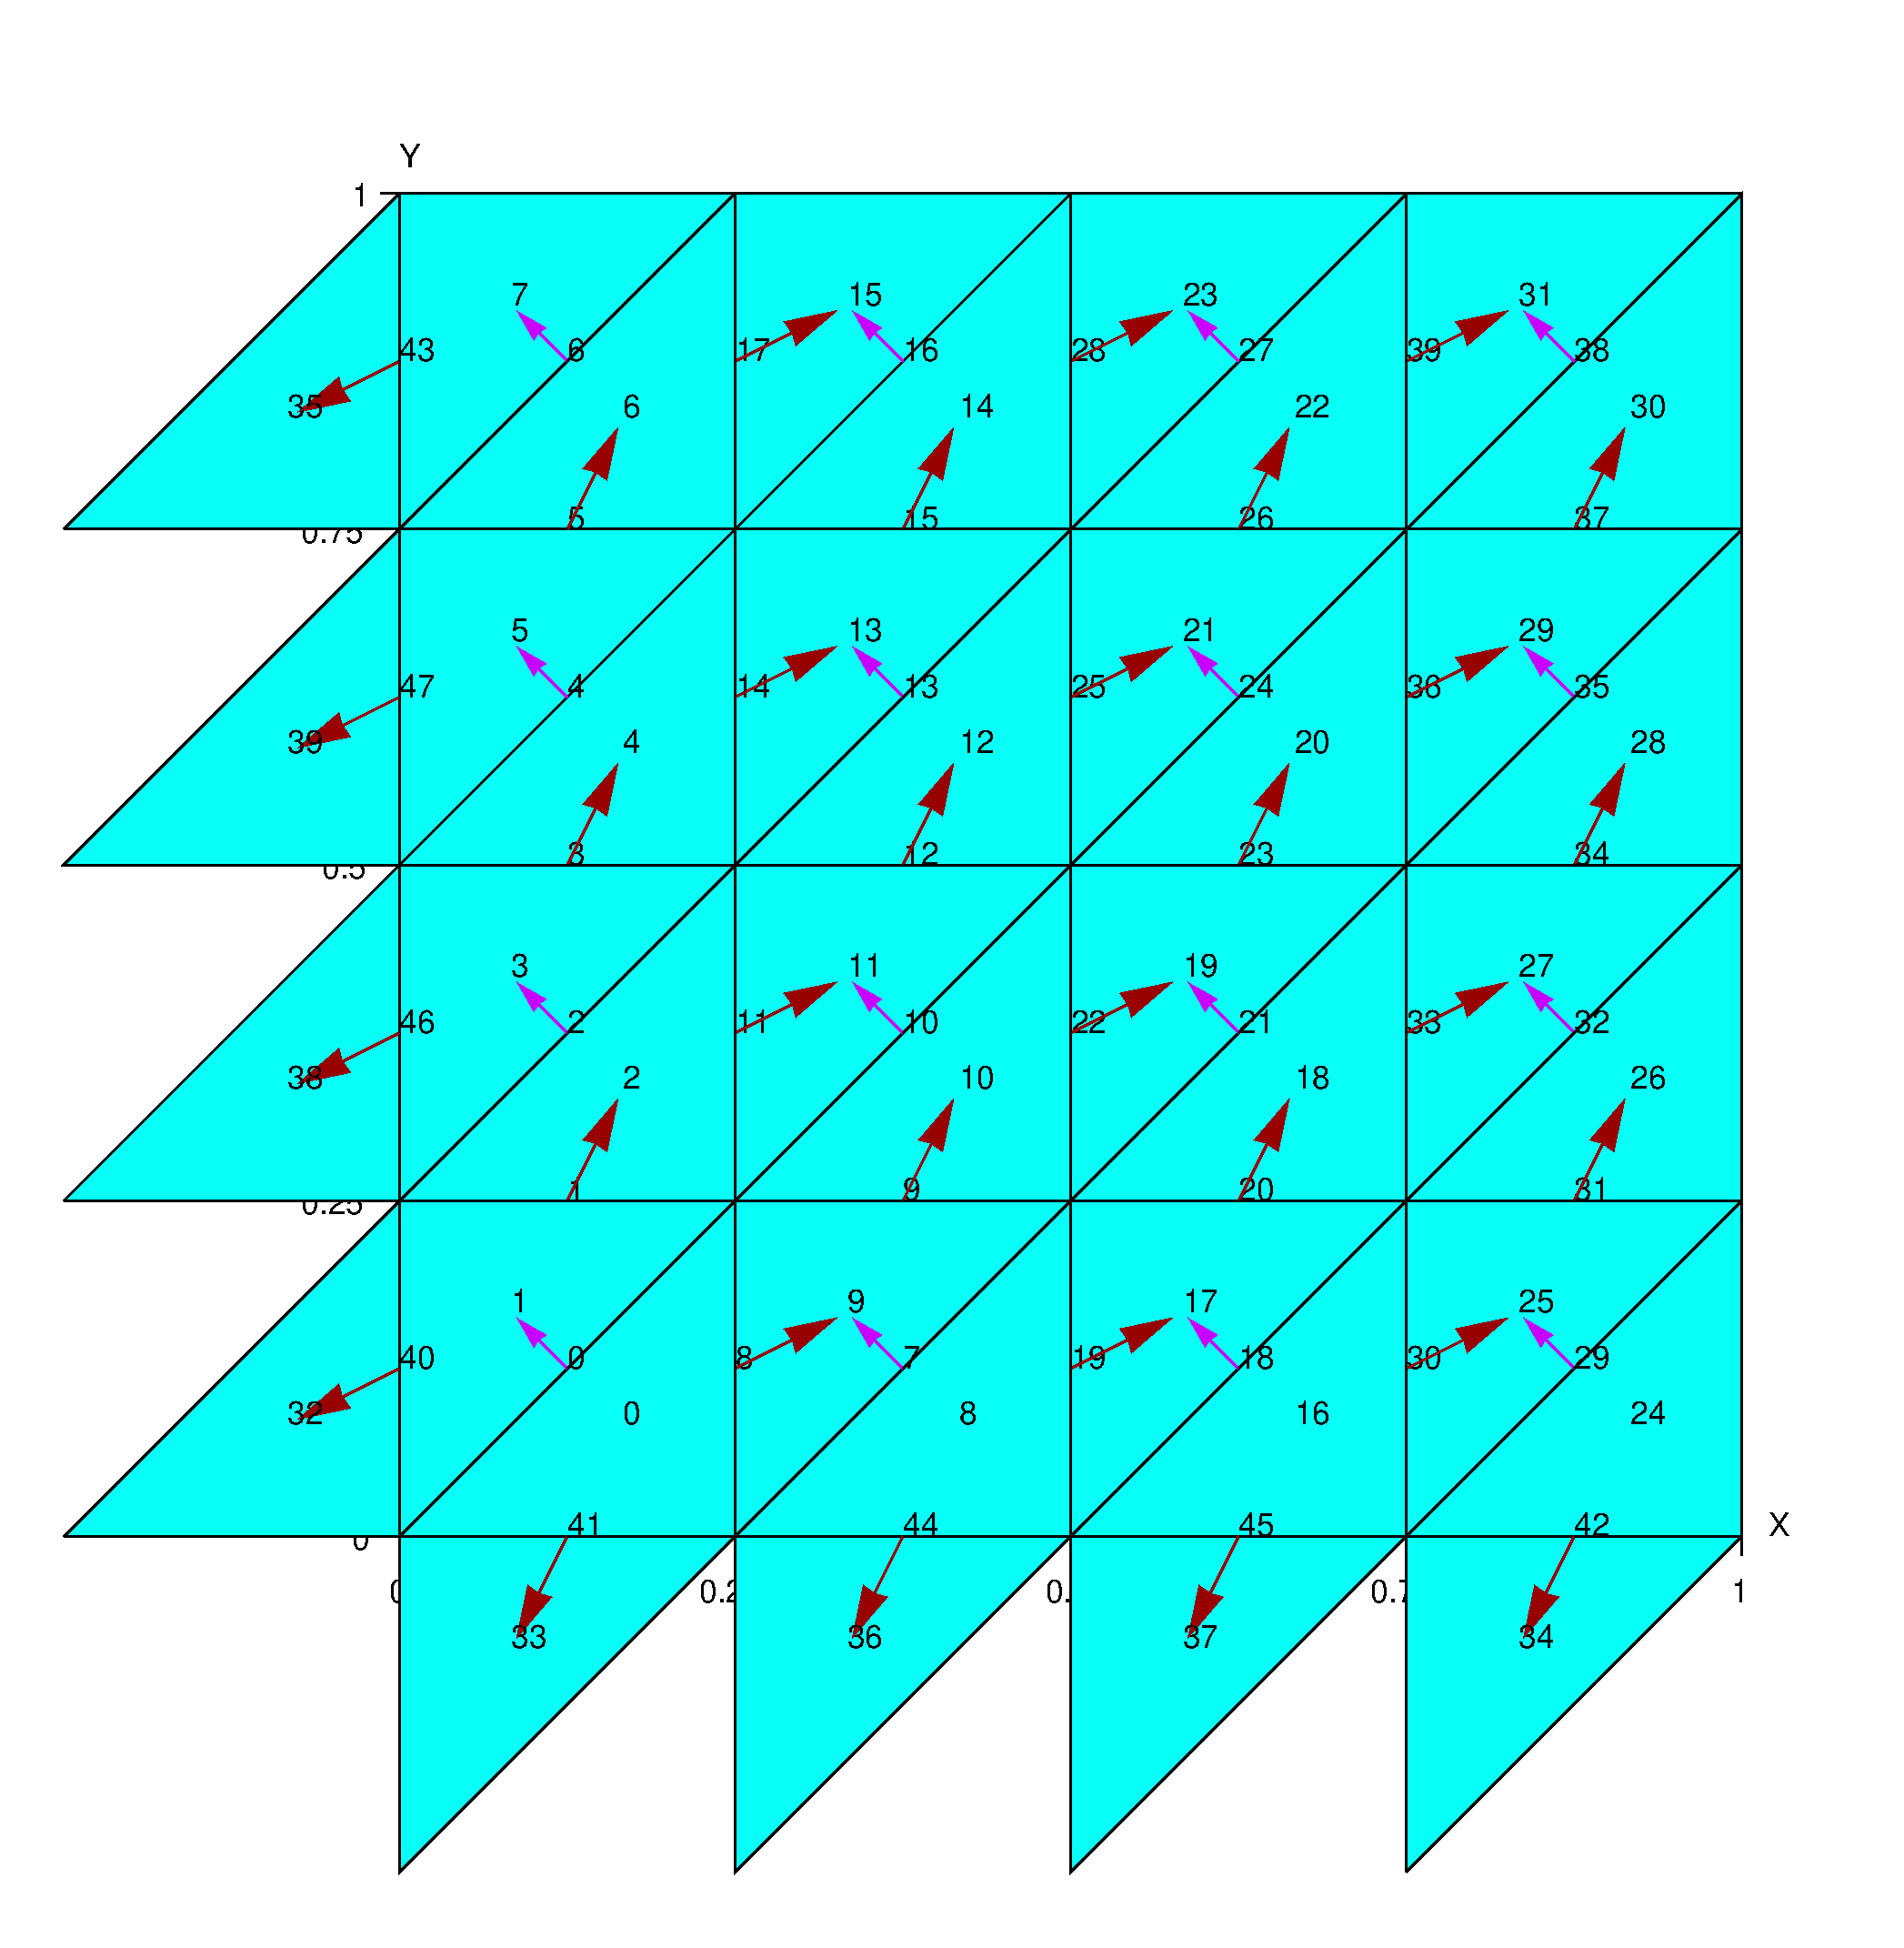
\includegraphics{SquareMesh2.pdf}}
\caption{Straddlers. 
         Integers inside panels denote panel indices.
         Indices lying atop edges denote RWG basis-function indices.
         Arrows indicate directions of current flow.}
\label{StraddlerFigure}
\end{center}
\end{figure}
%####################################################################%

\subsubsection{Evaluation of surface currents within the unit cell}

When evaluating the $\vb K$ and $\vb N$ surface-current 
distributions at panels that border the upper or right edges 
of the unit-cell mesh, we have to be careful to account for the 
contribution of straddlers. 

For example, consider evaluating the electric surface current at 
points $\vb x$ inside panel $\mc P_9$ in Figure (??) %\ref{Mesh3x3}.
There are three RWG basis functions that contribute to the current
at this point: $\vb b_7$, $\vb b_9,$ and the periodic image of 
$\vb b_2$:

\subsubsection{Relations between BEM matrix elements}

Looking at Figure \ref{StraddlerFigure}, it seems 
obvious that BEM matrix elements between the pair of 
basis functions
$\{\vb b_2, \vb b_{24}\}$ will be identical to those
between the pair 
$\{\vb b_4, \vb b_{27}\}$. (This much would be 
true even if we \textit{weren't} talking about
periodic geometries.)

Slightly less obvious is that matrix elements between
the pair $\{\vb b_6, \vb b_18\}$ will \textit{also}
be related to matrix elements between the above two
pairs---in fact, the elements will be \textit{identical}
for $\KB=0$ and will differ by only a phase factor
for $\KB\ne 0$. Let's now derive this relationship.

Let $\vb L$ be a lattice vector and suppose
$\{\vb b_\alpha, \vb b_\beta\}$ and
$\{\vb b_{\alpha^\prime}, \vb b_{\beta^\prime}\}$
are two RWG basis functions that are identical except 
for translation through $\vb L$, i.e. we have
%====================================================================%
\numeq{DisplacedRWG}
 { \vb b_\beta(\vb x) = \vb b_\beta^\prime(\vb x - \vb L).
 }
%====================================================================%
Examples of basis-function pairs in the mesh of Figure 
\ref{StraddlerFigure}, for which this condition is satisfied 
include
$$\begin{array}{lclclcl}
  \beta&=&2, \qquad \beta^\prime
  \end{array}
$$

\begin{align*}
\end{align*}
